%This work is licensed under the Creative Commons
%Attribution-ShareAlike 4.0 International License. To view a copy of
%this license, visit http://creativecommons.org/licenses/by-sa/4.0/ or
%send a letter to Creative Commons, PO Box 1866, Mountain View, CA
%94042, USA.

%This work is licensed under the Creative Commons
%Attribution-ShareAlike 4.0 International License. To view a copy of
%this license, visit http://creativecommons.org/licenses/by-sa/4.0/ or
%send a letter to Creative Commons, PO Box 1866, Mountain View, CA
%94042, USA.

%\documentclass[gray,handout, pdftex, 11pt]{beamer}
%\documentclass[handout, pdftex, 11pt]{beamer}

\documentclass[pdftex, 11pt]{beamer}

\usepackage[utf8]{inputenc}
\usepackage[T1]{fontenc}
\usepackage{lmodern}
%\usepackage[italian]{babel}
\usepackage{graphicx}
\usepackage{listings}
\usepackage{microtype}
\usepackage{acronym}
\usepackage{array}
\usepackage{tikz}
\usetikzlibrary{shapes, chains, scopes, shadows, positioning, arrows,
  decorations.pathmorphing, calc}

\colorlet{c1}{green!20}
\colorlet{c2}{blue!10}
\colorlet{drawColor}{black!50}
\colorlet{commentColor}{green!70!black!90}

\tikzstyle{oval}=[ellipse, align=center, drop shadow, draw=drawColor, fill=white]
\tikzstyle{rect}=[rectangle, rounded corners=2pt, align=center, drop
shadow, draw=drawColor, fill=white]
\tikzstyle{comment}=[text=commentColor,font=\itshape]
\tikzstyle{textLab}=[]
\tikzstyle{arrow}=[->, very thick, >=stealth', draw=black!80]
\tikzstyle{darrow}=[->, dash pattern=on 3pt off2pt, very thick, >=stealth', draw=black!80]
\tikzstyle{fStartEnd}=[ellipse, align=center, drop shadow, draw=drawColor, fill=white]
\tikzstyle{fInput}=[trapezium, trapezium left angle=70, trapezium right angle=110,
align=center, drop shadow, draw=drawColor, fill=white]
\tikzstyle{fProcess}=[rectangle, align=center, drop shadow, draw=drawColor, fill=white]
\tikzstyle{fSelection}=[diamond, shape aspect=3, align=center, drop
shadow, draw=drawColor, fill=white]
\tikzstyle{fOutput}=[tape, tape bend top=none, align=center, drop shadow, draw=drawColor, fill=white]
\tikzstyle{mem}=[rectangle, align=center, draw=drawColor, fill=white]
\tikzstyle{clo}=[cloud, aspect=2, align=center, drop shadow, draw=drawColor, fill=white]

\lstdefinestyle{customc}{
   language=C,
   % basicstyle=\small\ttfamily\bfseries,
   basicstyle=\ttfamily,
   keywordstyle=\color{blue}\ttfamily,
   stringstyle=\color{red}\ttfamily,
   commentstyle=\color{green}\ttfamily,
   morecomment=[l][\color{magenta}]{\#},
   % breaklines=false,
    breaklines=true, breakatwhitespace=false,
   frameround=fttt,
   frame=trBL,
   backgroundcolor=\color{yellow!20},
   numbers=left,
   stepnumber=1,    
   firstnumber=1,
   numberfirstline=true,
   numberstyle=\tiny\color{black!50},
   xleftmargin=2em,
   framexleftmargin=1.5em
   % linewidth=8cm,
}

\lstnewenvironment{cblock}[1][]
{
  \lstset{
    style=customc,
    #1
  }
}{}

\newcommand{\cfile}[2][]{
  \lstinputlisting[style=customc, #1]{#2}
}

\definecolor{links}{HTML}{2A1B81}
\hypersetup{colorlinks,linkcolor=links,urlcolor=links}

\definecolor{links}{HTML}{2A1B81}
\hypersetup{colorlinks,linkcolor=,urlcolor=links}


\mode<presentation>{
  %-------------------------1
  \usetheme{Boadilla}
  \usecolortheme{beaver}
  %-------------------------1
  %-------------------------2
  %\usetheme{Goettingen}
  %\usecolortheme{sidebartab}
  %-------------------------2
  %\useoutertheme[right]{sidebar}
  %\usefonttheme{default}
  \setbeamercovered{transparent}
  %\setbeameroption{show notes on second screen=right}
  \setbeamertemplate{navigation symbols}{}
  \setbeamertemplate{footline}{}

  \bibliographystyle{abbrv}  
  %\renewcommand\bibfont{\scriptsize}
  \setbeamertemplate{bibliography item}{\textbullet}
  \setbeamertemplate{itemize item}{\checkmark}
  \setbeamertemplate{itemize subitem}{-}
  \setbeamertemplate{enumerate items}[default]
  \setbeamertemplate{sections/subsections in toc}[square]
}

\subtitle{Logical Computational Thinking}
\institute[Tecnológico de Monterrey]{
  
\includegraphics[width=5cm]{img/logoTEC.jpg}\\[5mm]
  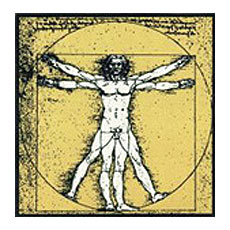
\includegraphics[width=1cm]{img/logoLEO.jpg}
  Scuola Leonardo Da Vinci (Firenze)
}

\author[Stefano Martina]{
  %\\[0.2cm]
  \textbf{Stefano MARTINA}\\
  {\small stefano.martina@gmail.com}
}

\titlegraphic{\tiny
  \href{http://creativecommons.org/licenses/by-sa/4.0/}{
\includegraphics[width=1cm]{img/logoCC.png}}
  This work is licensed under a
  \href{http://creativecommons.org/licenses/by-sa/4.0/}{Creative
    Commons Attribution-ShareAlike 4.0 International License}.}


\title[Lesson 3]{\textbf{Lesson 3 - Compiling a \C\ program}}
\date[14/9/15]{\flushright 14 September 2015}

\begin{document}

\begin{frame}[plain]
  \titlepage
\end{frame}

\begin{frame}
  \frametitle{\texttt{gcc} compiler for GNU/Linux}
  \begin{itemize}
  \item If you use Linux probably you have already gcc installed \rotatebox[origin=c]{270}{:)}
  \end{itemize}
\end{frame}

\begin{frame}
  \frametitle{\texttt{gcc} compiler for Mac}
  \begin{block}{Install}
    \begin{enumerate}
    \item Go to \url{https://developer.apple.com/downloads/};
    \item provide authentication, and if needed accept the agreement;
    \item search \alert{command line tools} on the left box;
    \item double click on \alert{Command line tools (...) for Xcode
        6.4};
    \item download \alert{dmg} file (click on the filename on the right);
    \item double click on the \alert{dmg} and then double
      click on the \alert{pkg} inside it;
    \item follow the installation instructions.
    \end{enumerate}
  \end{block}
\end{frame}

\begin{frame}
    \begin{block}{First use}
    \begin{enumerate}
    \item Open a terminal;
    \item type \alert{\texttt{sudo gcc -v}};
    \item provide authentication;
    \item read license, with \alert{space}, and agree, typing
      \alert{\texttt{agree}} at the end (attention not to press to
      much spaces).
    \end{enumerate}
  \end{block}
  \begin{block}{Text editor}
    \begin{itemize}
    \item A famous text editor for mac is \alert{TextMate} (version
      2.0), you can download it here: \url{https://macromates.com/download};
    \item another nice text editor is \alert{Atom}: \url{https://atom.io}.
    \end{itemize}
  \end{block}
\end{frame}

\begin{frame}
  \frametitle{\texttt{gcc} compiler for Windows}
  \begin{block}{Install}
    \begin{enumerate}
    \item Go to \url{https://cygwin.com/install.html};
    \item download and run the corresponding \alert{exe} (32 or 64
      bits);
    \item select \alert{Install from internet} and all the default
      options;
    \item when prompted, select a near server like
      \alert{\texttt{http://bo.mirror.gar.it}};
    \item when the packages list appear click on the + left to
      \alert{texttt{devel}} and then on \alert{\texttt{skip}} on the
      left of \alert{\texttt{gcc-core}} package (the word
      \texttt{skip} will change to a version number);
    \item click \alert{\texttt{next}} and accept all the question,
      when finished installing select \alert{\texttt{finish}}.
    \end{enumerate}
  \end{block}
\end{frame}

\begin{frame}
  \small
  \begin{block}{First use}
    \begin{enumerate}
    \item Open Cygwin from programs or desktop;
    \item type \alert{\texttt{cd
          /cygdrive/c/Users/[YourName]/Documents}} and you will go on
      your documents directory;
    \item go to your preferred working folder where you have sources
      files (\alert{\texttt{ls}} for listing files and directories,
      \alert{\texttt{cd}} for changing directory, \alert{\texttt{tab}}
      autocomplete path);
    \item you can use the \alert{\texttt{gcc}} compiler from here.
    \end{enumerate}
  \end{block}
  \begin{block}{Optional}
    \begin{itemize}
    \item Programs compiled with \alert{\texttt{gcc}} inside Cygwin
      can be executed only inside Cygwin.
      If you want to compile native Windows programs select also
      \alert{\texttt{mingw-gcc-core}} package during cygwin installation
      (you can re-run a cygwin installation and add packages), and then
      compile sources using \alert{\texttt{i686-pc-mingw32-gcc}} instead
      of \alert{\texttt{gcc}}.
    \end{itemize}
  \end{block}
\end{frame}

\begin{frame}
  \begin{block}{Text editor}
    \begin{itemize}
    \item A famous code editor for windows is \alert{notepad++}, you can
      find it here: \url{https://notepad-plus-plus.org/download/};
    \item another nice editor is \alert{Atom}: \url{https://atom.io/}.
    \end{itemize}
  \end{block}  
\end{frame}

\begin{frame}
  \frametitle{Alternative \texttt{gcc} compiler for Windows}
  An alternative to CygWin, maybe easier to use, is
  \alert{MinGW}. With that you can call \texttt{gcc} directly from the
  Windows command prompt.
  \begin{block}{Install}
    \tiny
    \begin{enumerate}
    \item go to \alert{\url{http://www.mingw.org/}};
    \item click on \alert{\texttt{download installer}} and execute it;
    \item follow the instruction and select default options;
    \item when asked for packages select \alert{\texttt{mingw32-base}}
      under \texttt{Basic Setup};
    \item click \alert{\texttt{apply changes}} under
      \alert{\texttt{installation}} menu, close the packet manager after;
    \item right-click on your ``My Computer'' icon and select
      ``Properties'';
    \item click on the ``Advanced'' tab, then on the ``Environment
      Variables'' button;
    \item you should be presented with a dialog box with two text
      boxes. The top box shows your user settings. The PATH entry in
      this box is the one you want to modify. Note that the bottom
      text box allows you to change the system PATH variable. You
      should not alter the system path variable in any manner, or you
      will cause all sorts of problems for you and your computer!
    \item click on the PATH entry in the TOP box, then click on the
      ``Edit'' button, if PATH don't exists click on ``new'' and create
      it;
    \item scroll to the end of the string and at the end add
      ``\alert{\texttt{;C:\textbackslash\textbackslash
          MinGW\textbackslash\textbackslash bin}}'' (if the string is empty don't
      insert the ``;''), in any case don't delete the possibly existing
      string;
    \item press OK -> OK -> OK.
    \end{enumerate}
  \end{block}
\end{frame}

\begin{frame}
  \begin{center}
    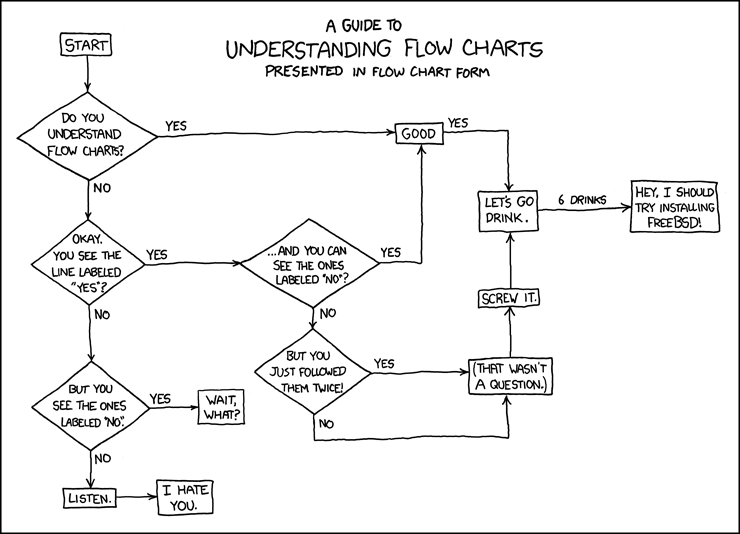
\includegraphics[width=\textwidth]{flow_charts.png}
  \end{center}
\end{frame}
\end{document}
